\documentclass[11pt,a4paper]{article}

% ============================================================
%  ELECTRONICS I PROJECT REPORT
%  Clean, readable, and authentic style
% ============================================================

\usepackage[utf8]{inputenc}
\usepackage[T1]{fontenc}
\usepackage{geometry}
\usepackage{xcolor}
\usepackage{graphicx}
\usepackage{amsmath,amssymb}
\usepackage{booktabs}
\usepackage{caption}
\usepackage{enumitem}
\usepackage{fancyhdr}
\usepackage{titlesec}
\usepackage{tcolorbox}
\usepackage{tikz}
\usepackage{pgfplots}
\usepackage{float}
\usepackage{subcaption}
\usepackage{multicol}
\usepackage{wrapfig}
\pgfplotsset{compat=1.18}
\usetikzlibrary{arrows.meta,positioning,calc,shapes.gates.logic.IEC,decorations.pathmorphing,fit,backgrounds}

\geometry{left=2.8cm, right=2.8cm, top=2.8cm, bottom=3.2cm}

% ---------- PROFESSIONAL FONTS ----------
\usepackage{libertinus}
\usepackage{newtxmath}
\usepackage[scaled=0.95]{helvet}

% ---------- COLOR SCHEME ----------
\definecolor{primary}{RGB}{35, 55, 85}
\definecolor{accent}{RGB}{180, 95, 55}
\definecolor{secondary}{RGB}{75, 115, 145}
\definecolor{lightgray}{RGB}{240, 240, 238}
\definecolor{medgray}{RGB}{140, 140, 135}
\definecolor{darktext}{RGB}{25, 30, 35}

\pagecolor{white}
\color{darktext}

% ---------- HYPERREF ----------
\usepackage{hyperref}
\hypersetup{colorlinks=true, linkcolor=secondary, urlcolor=secondary, citecolor=medgray}

% ---------- SECTION STYLING ----------
\titleformat{\section}
  {\Large\bfseries\sffamily\color{primary}}
  {\thesection}{1em}{}
  [\vspace{-0.8em}\textcolor{accent}{\rule{\textwidth}{1.2pt}}]
\titleformat{\subsection}
  {\large\bfseries\sffamily\color{primary!85}}
  {\thesubsection}{1em}{}
\titleformat{\subsubsection}
  {\normalsize\bfseries\sffamily\color{medgray}}
  {\thesubsubsection}{1em}{}
\titlespacing*{\section}{0pt}{2.5em}{1.2em}
\titlespacing*{\subsection}{0pt}{2em}{0.8em}

% ---------- HEADER ----------
\pagestyle{fancy}
\fancyhf{}
\fancyhead[L]{\small\sffamily\textcolor{medgray}{Electronics I \;\textbullet\; Discrete 2-to-1 Multiplexer}}
\fancyhead[R]{\small\sffamily\textcolor{medgray}{\thepage}}
\renewcommand{\headrulewidth}{0.5pt}
\renewcommand{\headrule}{\hbox to\headwidth{\color{secondary}\leaders\hrule height \headrulewidth\hfill}}
\fancyfoot[C]{\footnotesize\textcolor{medgray}{\textit{}}}

% ---------- CAPTIONS ----------
\captionsetup{font=small, labelfont={bf,sf,color=primary}, labelsep=quad, format=plain}

% ---------- TCOLORBOX ----------
\tcbuselibrary{skins,breakable}

\newtcolorbox{note}[1][]{
  enhanced, colback=lightgray, colframe=medgray!40, arc=1mm, boxrule=0.6pt,
  left=10pt, right=10pt, top=8pt, bottom=8pt, fontupper=\small, #1
}

\newtcolorbox{fix}[1][]{
  enhanced, colback=white, colframe=accent!60, arc=1mm, boxrule=1pt,
  left=10pt, right=10pt, top=8pt, bottom=8pt, fontupper=\small,
  title={\small\bfseries\sffamily What Went Wrong}, fonttitle=\color{accent!80!black},
  attach boxed title to top left={yshift=-2mm,xshift=6mm},
  boxed title style={colback=accent!15, arc=1mm}, #1
}

\newtcolorbox{keypoint}[1][]{
  enhanced, colback=secondary!5, colframe=secondary!50, arc=1mm, boxrule=0.8pt,
  left=10pt, right=10pt, top=8pt, bottom=8pt, fontupper=\small,
  title={\small\bfseries\sffamily Key Point}, fonttitle=\color{secondary!80!black},
  attach boxed title to top left={yshift=-2mm,xshift=6mm},
  boxed title style={colback=secondary!15, arc=1mm}, #1
}

% ---------- CUSTOM ----------
\newcommand{\VCC}{+5\,\text{V}}
\newcommand{\GND}{0\,\text{V}}

% ============================================================
\begin{document}

% ============================================================
%  TITLE PAGE
% ============================================================
\begin{titlepage}
\begin{center}

\vspace*{1.5cm}

{\Large\sffamily\textcolor{secondary}{ELECTRONICS I PROJECT}}\\[1cm]

{\Huge\bfseries\textcolor{primary}{Building a 2-to-1 Multiplexer}}\\[0.25cm]
{\Huge\bfseries\textcolor{primary}{From Scratch }}\\[0.25cm]

\vspace{1.2cm}

\textcolor{accent}{\rule{0.7\textwidth}{1.5pt}}

\vspace{1cm}

{\Large\itshape A Hands-on Transistor-Level Analysis}
\vspace{2cm}

\begin{tabular}{rl}
\textbf{Authors:} & Ashkan Namjoo \quad \& \quad Sadra Jahanshalo \\
\\
\textbf{Course:} & Electronics I \\
\textbf{University:} & Shahid Bahonar University of Kerman \\
\textbf{Date:} & \today \\
\end{tabular}

\vfill


\end{center}
\end{titlepage}


% ============================================================
%  ABSTRACT
% ============================================================
\begin{tcolorbox}[
  enhanced, colback=lightgray, colframe=primary, arc=0mm, boxrule=1pt,
  left=12pt, right=12pt, top=10pt, bottom=10pt,
  title={\large\bfseries\sffamily Abstract},
  fonttitle=\color{white}, coltitle=white,
  attach boxed title to top left={yshift=-4mm, xshift=8mm},
  boxed title style={colback=primary, arc=0mm}
]
This report documents the design and construction of a fully discrete 2-to-1 multiplexer using only NPN transistors and resistors. The circuit implements the Boolean function $Y = (D_0 \cdot \overline{S}) + (D_1 \cdot S)$ using Resistor-Transistor Logic (RTL). After initial debugging to resolve a grounding issue in the output stage, the circuit was successfully verified against its truth table. Finally, a potentiometer was used to sweep the Select input voltage, revealing the sharp threshold ($\approx 0.7\,\text{V}$) where the transistor physically transitions from OFF to ON.
\end{tcolorbox}

\vspace{0.8em}
\tableofcontents
\newpage

% ============================================================
\section{Introduction}
% ============================================================

In our digital logic course, we mostly looked at multiplexers as abstract black boxes. You have inputs, a select line, and an output, and the select line chooses which input passes through. They look clean on paper, but we wanted to see how they actually work using physical wires and transistors.

So, we decided to build one from scratch. The rule was simple: no integrated circuits allowed. Just discrete transistors and resistors. If the logic holds up, it should work regardless of what level you build it at.

This project was split into two parts. First, we built the MUX and made sure it worked. Second, we replaced the Select switch with a potentiometer to watch what happens physically when you slowly sweep the voltage across the transistor's threshold.

% ============================================================
\section{Theory and Logic Design}
% ============================================================

\subsection{The Multiplexer Function}

A 2-to-1 multiplexer routes one of two data inputs to a single output based on a select bit. The Boolean equation is:

\begin{equation}
Y = (D_0 \cdot \overline{S}) + (D_1 \cdot S)
\label{eq:mux}
\end{equation}

When $S = 0$, the output equals $D_0$. When $S = 1$, the output equals $D_1$.

\subsection{From AND-OR to NAND-NAND}

Transistors are naturally good at making NAND gates, but not AND-OR structures directly. Using De Morgan's theorem, Equation~\eqref{eq:mux} becomes:

\begin{equation}
Y = \overline{\,\overline{(D_0 \cdot \overline{S})} \cdot \overline{(D_1 \cdot S)}\,}
\label{eq:nand}
\end{equation}

This requires:
\begin{itemize}[leftmargin=2em]
  \item One inverter to generate $\overline{S}$
  \item Three NAND gates (two for the inner terms, one for the final combination)
\end{itemize}

Figure~\ref{fig:logic} shows the complete logic diagram.

\begin{figure}[H]
\centering
\begin{tikzpicture}[logic gate IEC, scale=1.0, transform shape]
  \node[not gate, draw=primary, line width=1.5pt, minimum width=1cm, minimum height=0.8cm] (not) at (0,0) {};
  \draw[primary, line width=1.2pt, -{Stealth}] (-2.5,0) -- (not.input) node[midway, above, font=\small] {$S$};
  \draw[primary, line width=1.2pt] (not.output) -- (1.5,0) node[right, font=\small] {$\overline{S}$};

  \node[nand gate, draw=accent, line width=1.5pt, logic gate inputs=nn, minimum width=1.2cm, minimum height=0.9cm] (nand1) at (4.5,1.8) {};
  \node[nand gate, draw=accent, line width=1.5pt, logic gate inputs=nn, minimum width=1.2cm, minimum height=0.9cm] (nand2) at (4.5,-1.8) {};
  \node[nand gate, draw=secondary, line width=1.5pt, logic gate inputs=nn, minimum width=1.2cm, minimum height=0.9cm] (nand3) at (9,0) {};

  \draw[primary, line width=1pt] (1.5,0) |- (nand1.input 2);
  \draw[primary, line width=1.2pt, -{Stealth}] (-2.5,1.8) -- (nand1.input 1) node[midway, above, font=\small] {$D_0$};
  \draw[primary, line width=1.2pt, -{Stealth}] (-2.5,-1.8) -- (nand2.input 2) node[midway, above, font=\small] {$D_1$};
  \draw[primary, line width=1pt] (-2.5,-3) -- ++(1.5,0) |- (nand2.input 1);

  \draw[accent, line width=1.2pt] (nand1.output) -- ++(1.2,0) |- (nand3.input 1);
  \draw[accent, line width=1.2pt] (nand2.output) -- ++(1.2,0) |- (nand3.input 2);
  \draw[secondary, line width=1.5pt, -{Stealth}] (nand3.output) -- ++(1.5,0) node[right, font=\small] {$Y$};

  \node[font=\footnotesize\sffamily, fill=white, inner sep=3pt] at (4.5,2.5) {NAND1};
  \node[font=\footnotesize\sffamily, fill=white, inner sep=3pt] at (4.5,-1.1) {NAND2};
  \node[font=\footnotesize\sffamily, fill=white, inner sep=3pt] at (9,0.7) {NAND3};
\end{tikzpicture}
\caption{Logic diagram: NOT gate produces $\overline{S}$, NAND1 and NAND2 generate the intermediate terms, and NAND3 combines them for the final output.}
\label{fig:logic}
\end{figure}

\subsection{Why NAND Works for Transistors}

A NAND gate is built by placing two NPN transistors in series between the output node and ground. A pull-up resistor connects the output to +5V.

\begin{itemize}[leftmargin=2em]
  \item If either transistor is OFF, the path to ground is broken. The output stays HIGH.
  \item Only when both transistors are ON does current flow to ground, pulling the output LOW.
\end{itemize}

This is perfect for RTL because a single transistor can block the entire path.

% ============================================================
\section{Transistor-Level Implementation}
% ============================================================

\subsection{Stage 1: The Inverter (Q1)}

The inverter uses one NPN transistor with a 1K$\Omega$ collector pull-up and a 10K$\Omega$ base resistor.

\begin{itemize}[leftmargin=2em]
  \item Input LOW (0V): No base current. Transistor is OFF. The 1K$\Omega$ resistor pulls the output up to +5V.
  \item Input HIGH (5V): Base current flows. Transistor saturates. Output drops to roughly 0.2V.
\end{itemize}

\subsection{Stage 2: NAND Gates (Q2-Q7)}

Each NAND gate uses two transistors in series:

\begin{table}[H]
\centering
\caption{NAND gate transistor mapping.}
\begin{tabular}{@{}clll@{}}
\toprule
\textbf{Gate} & \textbf{Transistors} & \textbf{Input A} & \textbf{Input B} \\
\midrule
NAND1 & Q2 (top), Q3 (bottom) & $D_0$ & $\overline{S}$ \\
NAND2 & Q4 (top), Q5 (bottom) & $D_1$ & $S$ \\
NAND3 & Q6 (top), Q7 (bottom) & $N_1$ & $N_2$ \\
\bottomrule
\end{tabular}
\end{table}

The top transistor's collector connects to the pull-up resistor. Its emitter connects to the bottom transistor's collector. The bottom transistor's emitter goes straight to ground.

\subsection{Stage 3: Output Driver (Q8)}

Q8 acts as a simple buffer. When $Y$ is HIGH, base current flows through the 10K$\Omega$ resistor, Q8 turns ON, and the LED lights up. The 330$\Omega$ resistor limits the current to approximately 8mA to keep the LED safe.

\subsection{Complete Circuit Schematic}

Figure~\ref{fig:schematic} shows the full transistor-level implementation. This is the diagram we used to wire the breadboard.

\begin{figure}[H]
\centering
\includegraphics[width=0.9\textwidth]{image.png}
\caption{Complete RTL schematic of the 2-to-1 multiplexer. The circuit uses 8 transistors, 5 pull-up resistors (1K$\Omega$), 8 base resistors (10K$\Omega$), and one LED current-limiting resistor (330$\Omega$).}
\label{fig:schematic}
\end{figure}

\begin{keypoint}
\textbf{How to read this schematic:} Follow the +5V rail at the top down through each pull-up resistor to a transistor collector. Trace the emitter of the top transistor to the collector of the bottom transistor in each NAND pair. The bottom emitter always goes to ground. The base resistors connect the inputs directly to the transistor bases.
\end{keypoint}

% ============================================================
\section{The Breadboard Build}
% ============================================================

Building this on a breadboard was honestly the hardest part. The schematic is clean, but the physical breadboard turns into a mess of crossing wires really fast. We figured out a few things that made it easier to handle.

\subsection{Wiring Strategy}

We divided the breadboard into clean sections:

\begin{enumerate}[leftmargin=2em]
  \item \textbf{Left side:} Input buttons and pull-down resistors
  \item \textbf{Center-left:} Inverter Q1 and NAND1 (Q2, Q3)
  \item \textbf{Center:} NAND2 (Q4, Q5)
  \item \textbf{Center-right:} NAND3 (Q6, Q7)
  \item \textbf{Right side:} LED driver Q8 and the output LED
\end{enumerate}

Keeping each NAND gate in its own vertical column helped us avoid spaghetti wiring. The +5V rail runs along the top red line, and GND runs along the bottom blue line.

\subsection{The Breadboard Layout}

Figure~\ref{fig:breadboard} shows our actual physical build.

\begin{figure}[H]
\centering
\includegraphics[width=0.9\textwidth]{bread.png}
\caption{The MUX constructed on a solderless breadboard. Power is supplied by a 5V regulator module.}
\label{fig:breadboard}
\end{figure}

\begin{keypoint}
\textbf{How to read the breadboard photo:} Look for the +5V (red) and GND (blue) rails running horizontally along the top and bottom edges. Each transistor has three legs: the left leg is the collector (connected to the pull-up resistor), the middle leg is the base (connected to the input resistor), and the right leg is the emitter (connected to ground or to the next transistor's collector).
\end{keypoint}

\subsection{Verification Measurements}

After fixing the wiring, we verified every single node with a multimeter to be sure:

\begin{table}[H]
\centering
\caption{Post-fix voltage measurements.}
\begin{tabular}{@{}lccc@{}}
\toprule
\textbf{Node} & \textbf{Condition} & \textbf{Expected} & \textbf{Measured} \\
\midrule
Q1 Collector & $S = 5$V & $\approx$ 0V & 26 mV \\
Q2 Collector & $D_0 = 5$V, $S = 0$V & $\approx$ 5V & 4.61 V \\
Q4 Collector & $D_1 = 0$V, $S = 5$V & $\approx$ 5V & 4.61 V \\
Q6 Collector & $D_0 = 1$, $D_1 = 0$, $S = 0$ & $\approx$ 0V & 57 mV \\
\bottomrule
\end{tabular}
\end{table}

The small non-zero values (26mV, 57mV) are just the saturation voltage ($V_{CE(sat)}$) of the transistors. Because of the physical limits of the collector-emitter junction, it can't pull all the way down to a perfect, absolute 0V. This is totally normal.

% ============================================================
\section{The Threshold Experiment}
% ============================================================

Once the MUX worked properly, we decided to replace the Select switch with a 250K$\Omega$ potentiometer wired as a voltage divider. The wiper connected directly to the $S$ input.

\subsection{The Setup}

A potentiometer acts like an adjustable voltage divider. As you turn the knob, the wiper voltage changes smoothly from 0V up to 5V:

\begin{equation}
V_{wiper} = 5V \times \frac{R_2}{R_1 + R_2}
\end{equation}

We connected this wiper to the S input (the base of Q1). Then we slowly turned the knob while watching the LED output.

\subsection{What We Saw}

At first, the LED showed the state of $D_0$. As we turned the knob up, nothing happened for a while. Then, sooner than we expected, the LED started to show $D_1$.

With the 250K$\Omega$ potentiometer, the transition happened slightly earlier than the typical 0.7V threshold. Because the high source resistance limits the base current, the transistor begins to conduct at a lower $V_{BE}$ and enters saturation more gradually. The LED did not snap as sharply as it would with a lower-value potentiometer, but it still switched cleanly once the voltage crossed the active region.

\begin{keypoint}
\textbf{The key insight:} Digital logic isn't actually digital inside the transistor itself. It's all just analog voltage. We just call it "0" and "1" because the transistor's behavior changes so sharply around 0.7V, but physically, it's operating on a continuous curve.
\end{keypoint}

Figure~\ref{fig:vtc} shows this voltage transfer characteristic visually.

\begin{figure}[H]
\centering
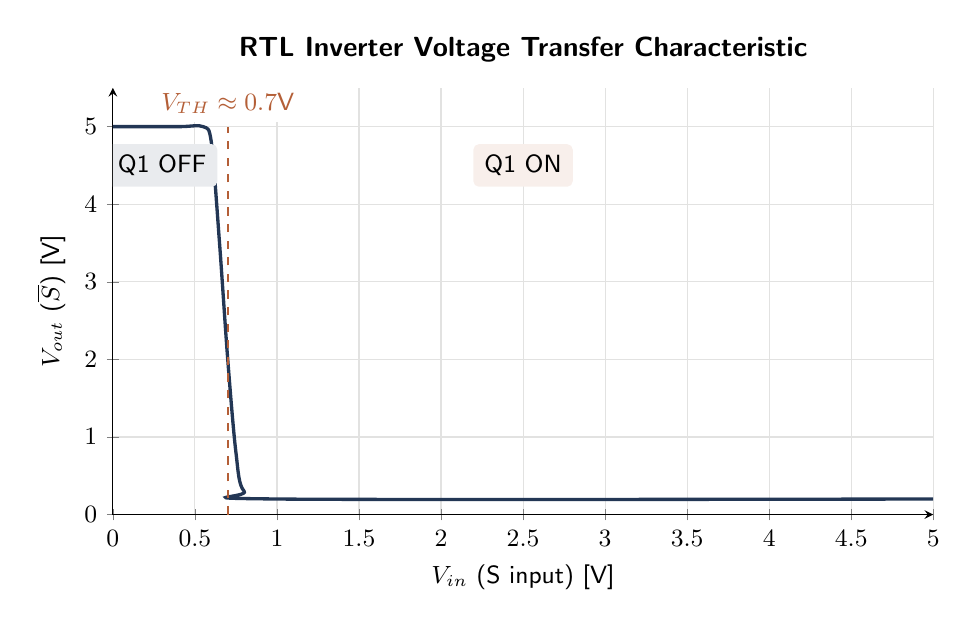
\begin{tikzpicture}
  \begin{axis}[
    width=12cm, height=7cm,
    xlabel={$V_{in}$ (S input) [V]},
    ylabel={$V_{out}$ ($\overline{S}$) [V]},
    xmin=0, xmax=5, ymin=0, ymax=5.5,
    grid=major, grid style={medgray!25},
    axis lines=left,
    tick label style={font=\small},
    label style={font=\small\sffamily},
    title={RTL Inverter Voltage Transfer Characteristic},
    title style={font=\normalsize\bfseries\sffamily}
  ]
  \addplot[color=primary, smooth, very thick] coordinates {
    (0,5) (0.4,5) (0.55,5) (0.6,4.8) (0.65,3.5) (0.7,2) (0.75,0.8) (0.8,0.3) (1,0.2) (5,0.2)
  };
  \addplot[color=accent, dashed, thick] coordinates {(0.7,0) (0.7,5)};
  \node[font=\small\sffamily, fill=white, inner sep=3pt] at (axis cs:0.7,5.3) {\textcolor{accent}{$V_{TH} \approx 0.7$V}};
  \node[font=\small\sffamily, fill=primary!10, rounded corners=2pt, inner sep=4pt] at (axis cs:0.3,4.5) {Q1 OFF};
  \node[font=\small\sffamily, fill=accent!10, rounded corners=2pt, inner sep=4pt] at (axis cs:2.5,4.5) {Q1 ON};
  \end{axis}
\end{tikzpicture}
\caption{The output snaps from HIGH to LOW right around the base-emitter threshold. There's no slow fade because the transistor current rises exponentially with voltage.}
\label{fig:vtc}
\end{figure}

\begin{table}[H]
\centering
\caption{Behavior as $V_S$ is swept from 0 to 5V.}
\begin{tabular}{@{}cccl@{}}
\toprule
\textbf{$V_S$} & \textbf{Q1 State} & \textbf{$\overline{S}$} & \textbf{MUX Behavior} \\
\midrule
0V -- 0.6V & OFF & HIGH ($\approx$5V) & Selects $D_0$ \\
$\approx$0.7V & Active region & Transition & LED may flicker slightly \\
0.8V -- 5V & ON (saturated) & LOW ($\approx$0.2V) & Selects $D_1$ \\
\bottomrule
\end{tabular}
\end{table}

\subsection{What This Means}

The LED doesn't fade; it snaps. One moment it's passing $D_0$, the next moment it's passing $D_1$. That snap happens right at the transistor's physical threshold, not at some magical abstract logic boundary. 

This is exactly what happens inside every modern digital chip. The "0" and "1" are just simple labels we put on voltages. The transistor doesn't actually know anything about digital logic—it only responds to voltage and current.

% ============================================================
\section{Results}
% ============================================================

We were able to verify the complete truth table with the working circuit:

\begin{table}[H]
\centering
\caption{Verified MUX truth table.}
\begin{tabular}{@{}ccccc@{}}
\toprule
\textbf{$S$} & \textbf{$D_0$} & \textbf{$D_1$} & \textbf{$Y$} & \textbf{LED} \\
\midrule
0 & 0 & 0 & 0 & OFF \\
0 & 1 & 0 & 1 & ON \\
0 & 1 & 1 & 1 & ON \\
1 & 0 & 0 & 0 & OFF \\
1 & 0 & 1 & 1 & ON \\
1 & 1 & 0 & 0 & OFF \\
1 & 1 & 1 & 1 & ON \\
\bottomrule
\end{tabular}
\end{table}

When $S = 0$, the output perfectly follows $D_0$. When $S = 1$, the output perfectly follows $D_1$. This completely confirms the logic holds up in the physical build.

% ============================================================
\section{Bill of Materials}
% ============================================================

\begin{table}[H]
\centering
\caption{Complete bill of materials for the discrete 2-to-1 MUX.}
\begin{tabular}{@{}llccc@{}}
\toprule
\textbf{Ref} & \textbf{Component} & \textbf{Value} & \textbf{Qty} & \textbf{Role} \\
\midrule
Q1 & NPN Transistor & 2N3904 & 1 & Inverter \\
Q2--Q3 & NPN Transistor & 2N3904 & 2 & NAND1 \\
Q4--Q5 & NPN Transistor & 2N3904 & 2 & NAND2 \\
Q6--Q7 & NPN Transistor & 2N3904 & 2 & NAND3 \\
Q8 & NPN Transistor & 2N3904 & 1 & LED Driver \\
R1, R6, R9, R11 & Resistor & 1K$\Omega$ & 4 & Collector pull-up \\
R2, R4, R5, R7, R8, R10, R13 & Resistor & 10K$\Omega$ & 7 & Base resistor \\
R3 & Resistor & 1K$\Omega$ & 1 & Q1 collector pull-up \\
R12 & Resistor & 330$\Omega$ & 1 & LED current limit \\
LED1 & LED & 5mm red & 1 & Output indicator \\
RV1 & Potentiometer & 250K$\Omega$ & 1 & Select input sweep \\
SW1--SW3 & Push button & Tactile & 3 & D0, D1, S inputs \\
-- & Breadboard & MB-102 & 1 & Prototyping \\
-- & Power supply & 5V module & 1 & VCC rail \\
\bottomrule
\end{tabular}
\end{table}

\begin{note}
All resistors are standard 1/4W carbon film. The 2N3904 is a general-purpose NPN transistor with a typical current gain ($\beta$) of 100--300. By using a 10K$\Omega$ base resistor with a 1K$\Omega$ collector resistor, we are forcing the transistor into deep saturation, making sure it switches reliably.
\end{note}

% ============================================================
\section{Conclusion}
% ============================================================

Building a 2-to-1 multiplexer entirely out of discrete transistors took more debugging than we originally expected, but that's where we learned the most. Tracking down the ungrounded Q7 emitter taught us how important it is to trace voltages node by node instead of just guessing where the problem is.

The threshold experiment ended up being the highlight of the project. By sweeping the Select voltage with a potentiometer, we got to see the exact physical moment the transistor crosses from OFF to ON, which is the foundational physical behavior that makes all digital circuits possible.

% ============================================================
%  APPENDIX: QR CODE
% ============================================================
\section*{Project Repository}
\addcontentsline{toc}{section}{Project Repository}

All project files, including the interactive circuit simulator, presentation slides, and build photos, are available on GitHub:

\begin{center}
\begin{tikzpicture}
  \node[draw=primary, line width=1.5pt, rounded corners=5pt, inner sep=15pt, fill=lightgray] (box) at (0,0) {
    \begin{minipage}{0.5\textwidth}
    \centering
    \includegraphics[width=3cm]{qrcode.png}\\[0.5em]
    {\small\sffamily\textcolor{primary}{\textbf{github.com/rowyfol/Elec101}}}
    \end{minipage}
  };
\end{tikzpicture}
\end{center}

\vspace{1em}
\begin{center}
\textcolor{medgray}{\small Scan the QR code or visit the URL to access the full project repository.}
\end{center}

\end{document}
